\chapter{Concept and Design}
\label{cha:conceptanddesign}

\section{Stop Location Detection}

<<<<<<< f11e91c57998b18cc4aaee81f3b2c9db990dea64
\subsection{Stop Detection for proactive localization based services}
\label{cha:stopdet_proactive}
=======
We need to describe here what do we want to achieve, what do we mean by modeling and visualizing macroscopic movements etc - thus general architecture that we have 3 components, Stop Detection from telekom data based on movements and updates of "areas" in your mobile phone, Clustering of Stops to find most popular "stops" in the city, Graph Generation to find where do the people move and in what amount
>>>>>>> Documentation WIP

Analyzing different approaches for stop detection based on localization data (ref. \autoref{cha:introduction_appr_stopdet}), we decided to test and verify algorithms based on human behavior regarding mobility within the cities (ref. \autoref{cha:introduction_hummob}) and reusing the concept of Mobility Index (ref. \autoref{cha:introduction_mob_index_sect})). Stop Location Detection Algorithm have to be able not only identify the time of start stop, but also the stop location.
\\\\
The approaches also need to consider that because of the method of receiving data in proactive localization services, if human will enter a urban canyon, building or move underground his signal might need to be re-obtained after a movement to new area and this can take certain period of time, where points possibly can be spanned over mid-range/long distances. On the other hand, points received over a short distance might mean that person has been already moving with a good reception of signal.

\subsection{Mobility index based approach}
\label{cha:stopdet_mi}

In related works about mobility index discussed in \autoref{cha:introduction_mob_index_sect}, the approach to stop detection using mobility index is bound to the way the data is being sampled (handover from one GSM cell to another). The data is recorded whenever mobile device changes its GSM cell. In case of the approach discussed in this paper the situation is similar, however instead of GSM cells we have artificially created area around the location, and while new location is obtained at some distance after movement, new area might need to be updated and point is being recorded.
\\\\
In a populated area, the user can move from one area to another after several seconds or only after minutes. Thus, if within a certain
period of time (called mobility index time window) the user stays in the same area or changes the areas with small pace (mobility index is below certain threshold) it can be assumed that the user is immobile or approaching stop location and having stay somewhere within that time window (restricted area). 

\subsection{Human Behavior based approach}
\label{cha:stopdet_bh}

This approach targets the condition for movement between two points, which has to be satisfied, so that it can be considered as a stay within the certain distance. 
\\\\
The \autoref{cha:introduction_hummob} discusses, that in average, walking human is traveling with the speed of over 3km/h up to 5km/h. However for movement on long distances, user will most likely use city or private transport, and thus his speed can vary much in that time/distance period.
\\\\
This approach states, that if movement between two points has been recorded in very short distance - as described in \autoref{cha:stopdet_proactive}, and movement of speed is below a certain threshold, it might mean that user has stopped or has been moving very slowly within a restricted area, which is called possible stop for that location between these points. 
\\\\
For movements between points over mid/long distances recorded, user might have stopped at first location, moved with different speeds between points and continuing movement (proactive localization is used). As an example, movement over 6km, might require up to 10 minutes with transportation. If the user stopped at previous location for 20 minutes, thus, total movement between point took 30 minutes, which in average is around 12 km/h. Universal speed threshold is not able to detect stops in these kind of examples, since with travels over higher speeds with stop at previous location would result in relatively high average speed. 

\section{Clustering of Stops}

<<<<<<< f11e91c57998b18cc4aaee81f3b2c9db990dea64
Clustering can be described as "\textit{the task of grouping a set of objects in such a way that objects in the same group (called a cluster) are more similar (in some sense or another) to each other than to those in other groups (clusters)}" \cite{clustering}. 
\\\\
After our stop detection algorithm has detected the proper stops we want to perform some analysis on these. Our goal is to get the overall movement patterns of the population of a certain area, which means we are interested in \textbf{macroscopic} movements and not microscopic (individual) movement. If we would consider every individual our analysis algorithms would get fed with a lot of noise (outliers) which would make our data mining and prediction difficult and inaccurate. Meaning, \textit{Macroscopic Movements} are not interesting in tracking individuals but rather seeing the big picture.

 Once our clustering algorithm has been applied, and we have the overall picture, we can see which stops are most popular, where people are moving from them, and how long they stay at a certain location. One could then perform some interesting graph analysis on these locations, answering questions such as "what is the probability that a person moves from point \textit{A} to \textit{B}?", or "what is the average stop time at location \textit{A}?". 
 
 To achieve these clusters, which represents our interesting stop locations, we need to apply some clustering algorithm. There are different types of clustering (such as centroid, distribution, or density-based), and different algorithms with parameters that can be applied (such as K-means, DBScan, or OPTICS). However, they all work to achieve the same goal of structuring (clustering, grouping) similar objects and neglecting outliers from these groups. The algorithm and parameters are application sensitive and our choice will be handled in the \textit{evaluation} section.

\begin{figure}[!ht]
	\centering
	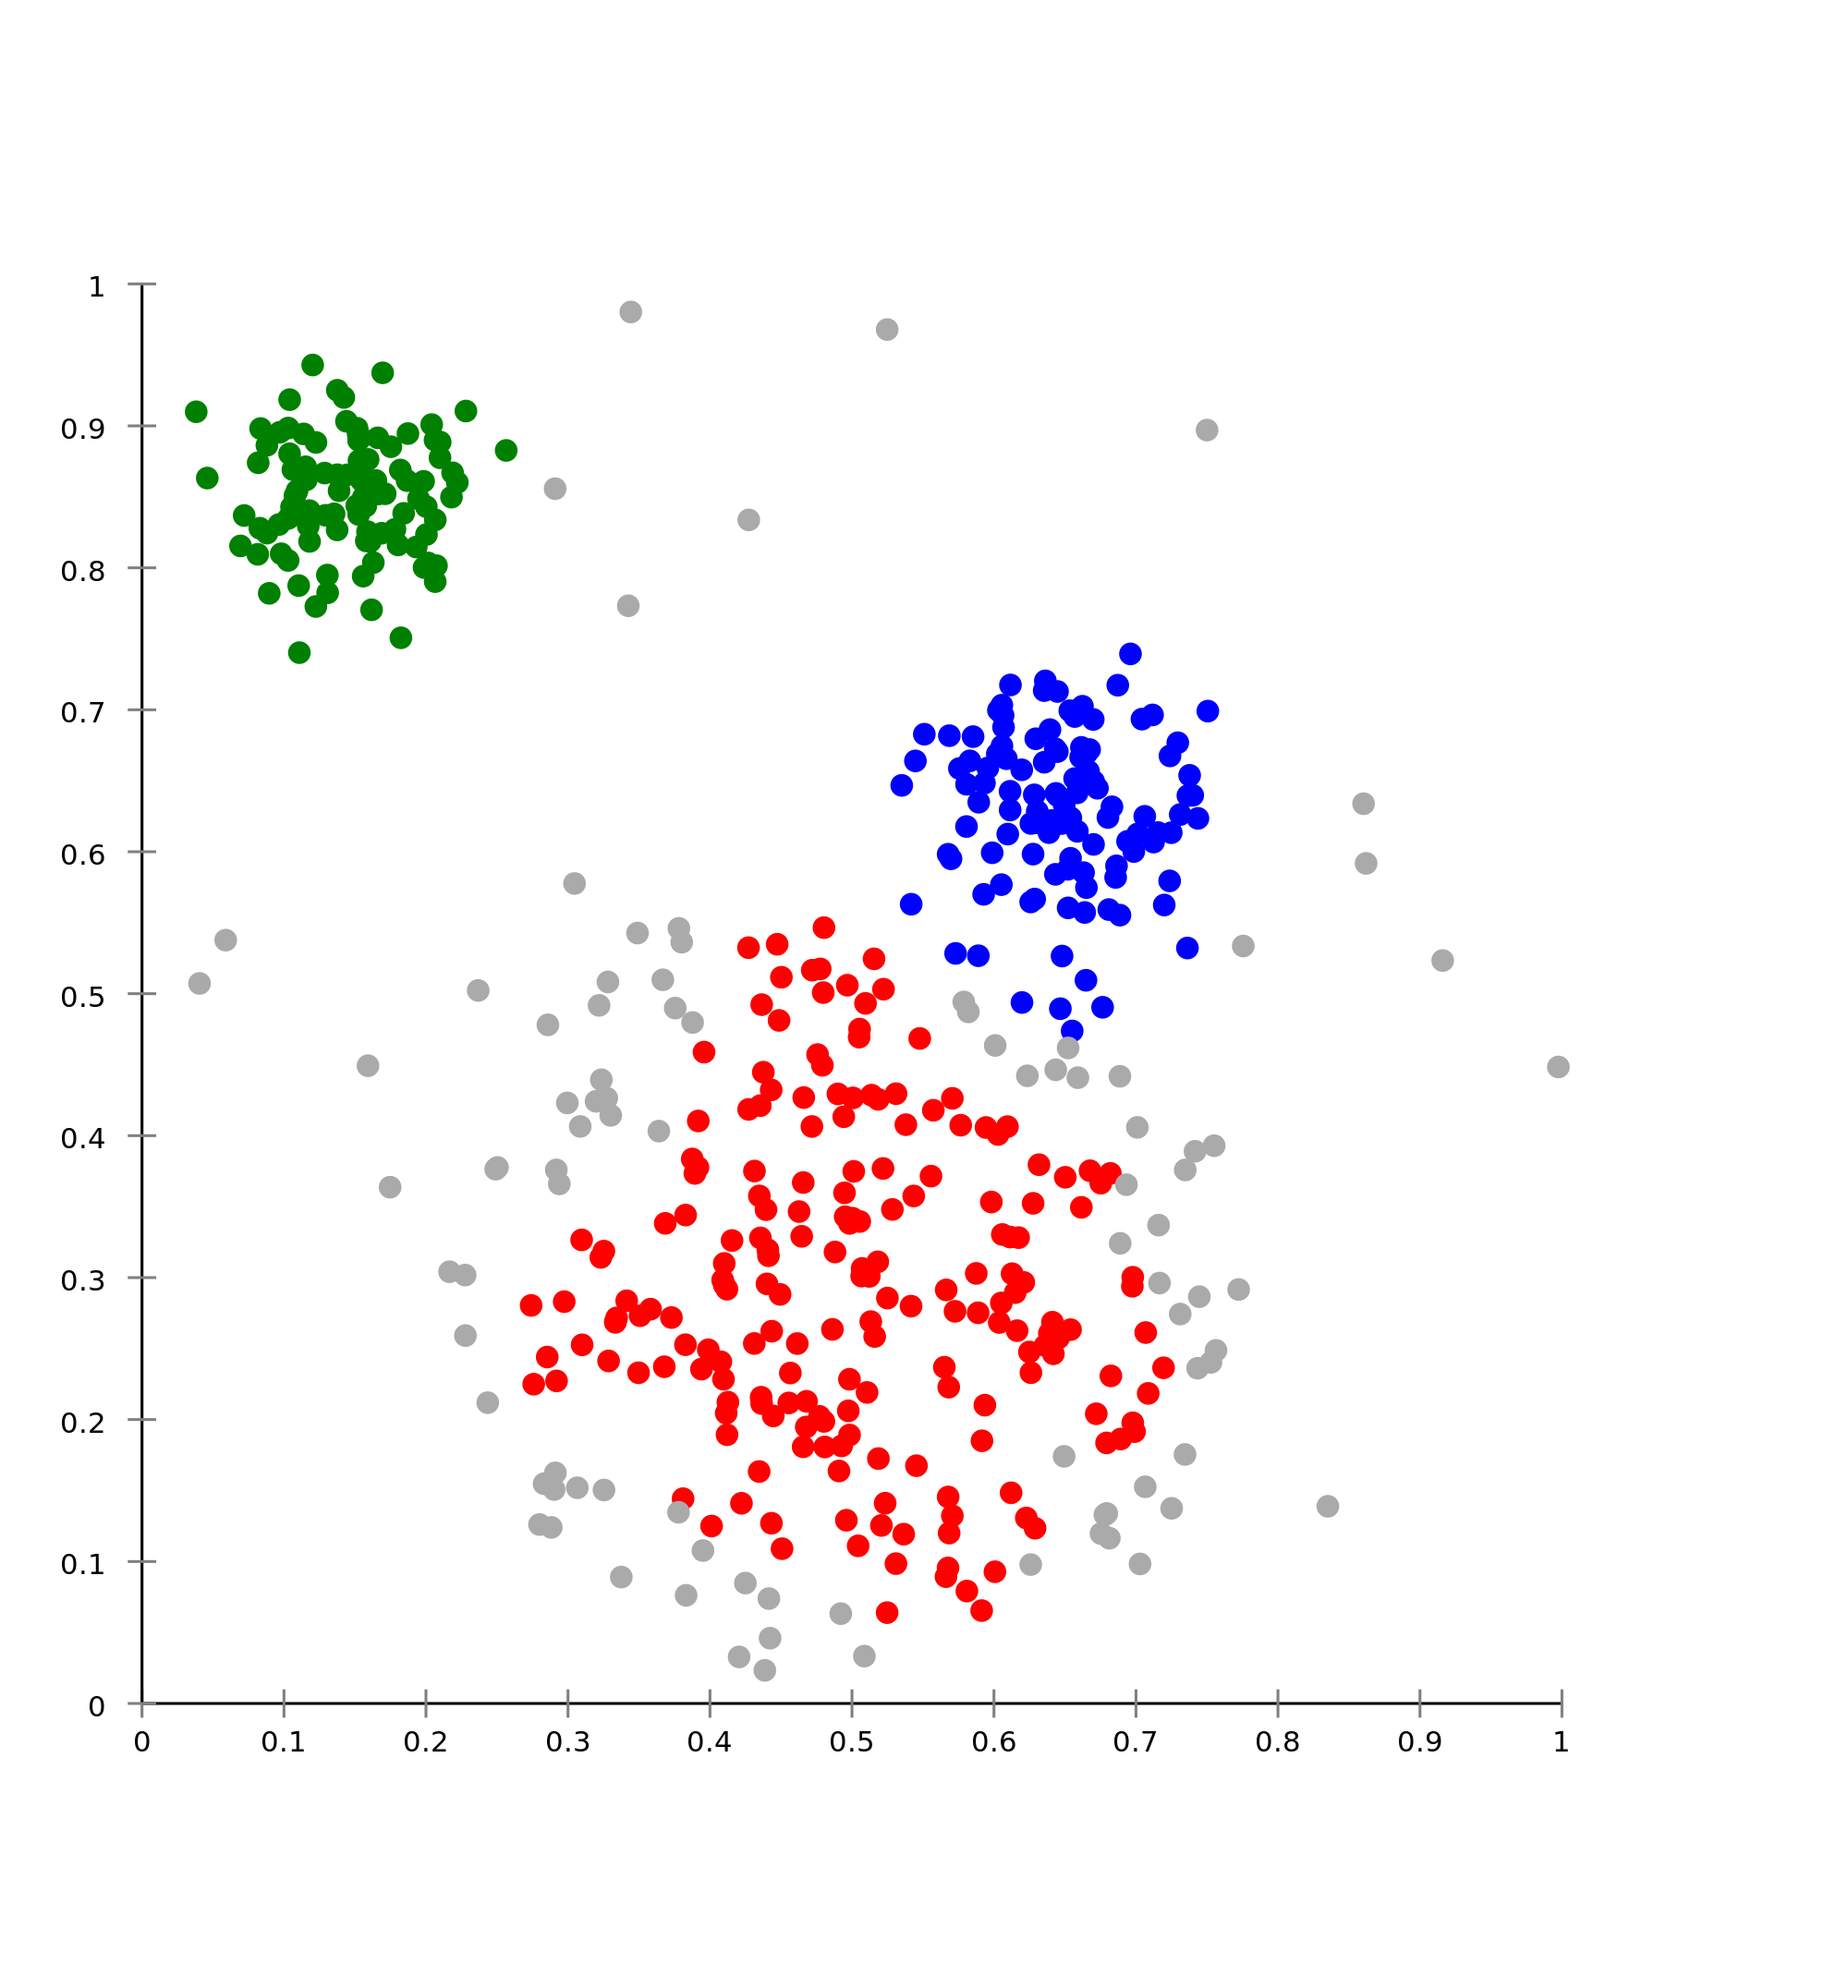
\includegraphics[width=0.6\textwidth]{images/clustering.png}
	\caption{ Clustering applied to a dataset. }
	\label{fig:clustering}
\end{figure} 

\FloatBarrier
\section{City Movements Graph}
\label{cha:movementsGraph}
Our target in this project is to identify popular locations and routes in a city and determine movement patterns of people. The stop points identified by the stop algorithm correspond to actual physical locations in the city with individual latitude and longitude values. These stop points are further clustered to identify places of interest in the city. A collection of such stop clusters, can be used to chart the movement of users in the city. 

The first step of creating a user movement graph is to create vertices and edges.It is important to outline how the vertices and edges have been selected for creating the city graph. Clusters generated by the DBSCAN algorithm are considered as vertices. If any user has more than two vertices, it is assumed that the user has moved between the successive points and an edge is constructed between them.  A directed graph is constructed from the set of edges and the direction of movement is considered from the first point going towards the next point in sequence.
\subsection{Graphical Representation and Analysis}
 We are using various characteristics of the graph like in- and out-degrees, strongly and weakly connected components, number of connected components, subgraphs and link-route incidence matrix \cite{kelly2008mathematics} for our analysis. We are also using the concept of Origin-Destination Matrix and obtaining Trip Count values between a pair of vertices. Correlations like these enable easy visualization of the movement patterns. 


\begin{figure}[!ht]
	\centering
	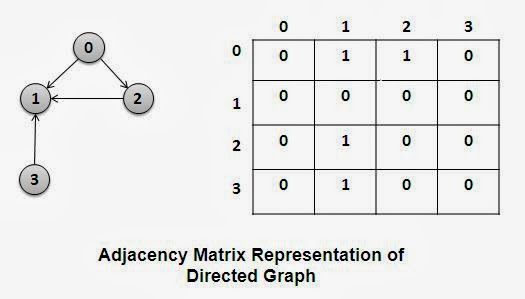
\includegraphics[width=0.6\textwidth]{images/AdjacencyMatrixExample.JPG}
	\caption{ Example: Matrix representation of a Directed Graph}
	\label{fig:Graph}
\end{figure} 

Pending: About OD Matrix, (cite in related works). About trip count and how it is used in case of creating a graphical network.

We can mark a vertex as either a sources or a destination of an edge. This incidence relation allows us to calculate the in-degrees and out-degrees of the vertices. Information like this can indicate many useful features, like most visited places in the city, by their high in/out-degrees. For example: the central train station or airport of a city will have a high in and out-degree, due to high number of people traveling to or from that place.

\FloatBarrier=======
\section{City Movements Graph}
One of the purposes of this project is to determine movement patterns of people and also identify popular locations and routes in a city. The "stop points" identified from the telekom data correspond to actual physical locations in the city with individual latitude and longitude values. These "stop points" are further clustered to identify places of interest in the city. These positions indicate places in a city where people are known to have stopped. Thus, these stop positions can be used to graphically represent movement of people in the city. When mapped to physical entities in a city, these stop positions correspond to an office, a University, a bus or train station, shopping mall etc. Thus movement pattern of inhabitants of a city can be determined.

\subsection {Purpose of graphical representation:} Representing user movement data graphically allows easy visualization and analysis of the data. Graphical representation of the movement patterns allows computation of different correlation and obtain conclusions?

\textbf{Selection of vertices and edges} It is important to outline how the vertices and edges were selected for graph creation.The clusters created out of the Stop points are represented as vertices. 
\textbf{Edge selection} For selecting edges, each user data is processed individually to determine the sequence of movement of a user from one vertex to the other. An edge is constructed between two vertices, if position of user changes from one cluster to another, with the assumption that user moved from the first cluster to the next one at some point of time.

<<<<<<< aca7e8935c264727bbcb343857b822a347891b47
<<<<<<< 35f005625e822ce66484e7d8466a14a805df8c98
The total list of edges is created with an aggregation of edges created for all users. In case of multiple occurrences of particular edges, the count is noted. For all other edges, number of occurrence is defaulted to 1.
>>>>>>> Documentation WIP
=======
The total list of edges is created with an aggregation of edges created for all users. In case of multiple occurrences of particular edges, the count is noted. For all other edges, number of occurrence is defaulted to 1. 
=======
The total list of edges is obtained by aggregating the edges created for all users. In case of multiple occurrence of an edges, the count is noted. For all other edges, number of occurrence is defaulted to 1. 
>>>>>>> Documentation WIP

\textbf{Intended goal}
>>>>>>> Documentation WIP
